% Dacier\cite{Dacier_1994, Dacier_1996}:
% privilege graph model assumes the probability to succeed in a given attack before time $t$ is described by an exponential distribution given by: $P(t) = 1-exp(-\lambda t) $  Transition rate $\lambda$ estimates the effort and time, with mean time for an attack to succeed given by $\frac{1}{\lambda}$.

% \textbf{MTTF}: $MTTF_k = T_k + \sum\limits_{1\in out(k)}P_{k1} ; P_{k1}=\lambda_{k1} \times T_k$


% The shortest path is the 
% \textbf{SP}: 


% Attack graphs are a widely studied field of information security modeling and a number of security metrics can be derived from them. Some authors\cite{Kordy_2013} attribute the first attack graph formalism to \cite{Weiss_1991} while others \cite{Ortalo_1999} credit \cite{Dacier_1994} with the discovery and still others\cite{Ramos_Lazar_Filho_Rodrigues_2017} state attack graphs were originally proposed by \cite{Phillips_Swiler_1998}. 

% Time Based: \cite{Ramos_Lazar_Filho_Rodrigues_2017}
% - privilege graph based
% \cite{Dacier_1994}: Privilege Graph based CTMC (Continuous Time Markov Chain), MTTF (Mean Time to Failure) , SP (Shortest Path)

% \cite{Ortalo_1999} METF (Mean Effort to Failure), TM (Total Memory), ML (MemoryLess), 

% - manually defined state-space based
% \cite{Almasizadeh_Azgomi_2013} countermeasures, resilience, MTSF (Mean Time to Security Failure) (Absorbing Markov Chain), 

% \cite{McQueen_Boyer_Flynn_Beitel_2006} MTTC (Mean Time to Compromise) with Compromise Graph, each component has an associated time to compromise, also Variable Length Markov Chain (in McQueen and Leversage) ** not validated

% Probability Based:: 
% \cite{Almasizadeh_Azgomi_2013} Steady-State security metric (derived from MTSF model, but transient instead of absorbing)

% \cite{Jha_Sheyner_Wing} reliability metric (probability of adversary NOT succeeding in an attack). Derived from CTMC with probability weighted edges. 

% \cite{Kanoun_Cuppens_Boulahia_Cuppens_Dubus_Martin_2009} Success Likelihood (SLH - CTMC based on AGs again)

% \cite{Li_Parker_Xu_2011} Renewal stochastic process to estimate probability that an attacker exploits a random vulnerability. 

% Model Based: 



% Surveys:

% \cite{Ramos_Lazar_Filho_Rodrigues_2017}\cite{Pendleton_Garcia-Lebron_Cho_Xu_2016}\cite{Verendel_2009}\cite{Anderson_Moore_2007}

% \cite{Verendel_2009} Reviews down selects 140 papers to 90 reviewed across multiple taxonomies. Finds CIA perspective under represented (11/90) in quantification methods. Economic is the most (61/90)

% \cite{Pendleton_Garcia-Lebron_Cho_Xu_2016} reviews attack graphs \cite{Phillips_Swiler_1998}, \cite{Sheyner_Haines_Jha_Lippmann_Wing_2002}, \cite{Ritchey_Ammann_2000}, \cite{Homer_Zhang_Ou_Schmidt_Du_Rajagopalan_Singhal_2013}, \cite{Jha_Sheyner_Wing},\cite{Cheng_Deng_Li_DeLoach_Singhal_Ou_2014}

Security metrics can be categorized by the area of cyber security to which they apply. In this respect, the security metric surveys available in recent literature are by nature focused narrowly on a specific subfield, such as cryptographic or software development lifecycle security metrics. We attempt to include these in a \textit{big-picture} view of the field of cyber security by classifying them under the general headings of the recently released Cyber Security Body of Knowledge\cite{Rashid_Chivers_Danezis_Lupu_Martin} depicted in Figure \ref{fig:cybok}. 


\begin{figure*}[ht]
\centering
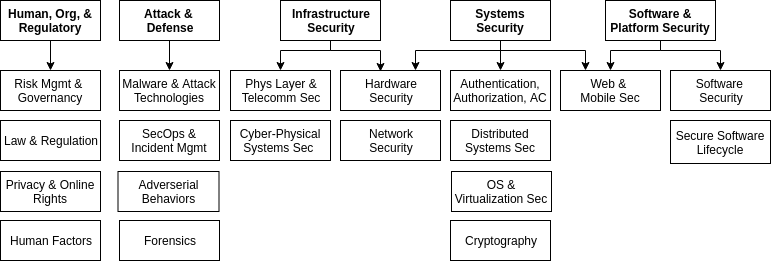
\includegraphics[width=.7\linewidth]{img/cybok_vert_no_heading.png}
\caption{Cyber Security Body of Knowledge - Key Areas}
\label{fig:cybok}
\end{figure*} 

\textbf{Human, Organizational, \& Regulatory} Vaughn’s taxonomy\cite{Vaughn_Henning_Siraj_2003} from 2003 is heavily influenced by federal, and in particular defense department, perspectives on information assurance metrics. The classification tree is heavy on the side of personnel and regulatory metrics compared to other surveys, and the categories draw from military concepts of operational readiness, threat identification, and target acquisition. In general these metrics are counts of the number of compliant systems, number of employees that have completed mandatory training, etc. The survey makes some important observations about properties common to all security metrics (objective/subjective, static/dynamic, qualitative/quantitative, etc). These are presented as binary values which may not be suitable for all metrics, but establishes the idea of universal attributes we can apply to any system.

\textbf{Systems} Ramos\cite{Ramos_Lazar_Filho_Rodrigues_2017} surveys model based network security metrics, which rely on a graph or tree structure representing the connectivity between system properties as input. These metrics are designated as Compliance based when a larger value indicates more security. Moment identifies if a measurement can be taken pre-deployment and remains static throughout operation, or if the metric is dynamic and should be measured repeatedly. Consistency distinguishes if the measured value relies on subjective human input or if its evaluation is objective. To compare with network performance metrics like latency or throughput, these security metrics are heavily influenced by subjective criteria. For example, the reliability based models make assumptions about an attacker’s success rate, level of effort, motivations, and capabilities that could change depending on who is filling in the weights. The primary classification in \cite{Ramos_Lazar_Filho_Rodrigues_2017} is by target. A metric can evaluate a Process (eg SSE-CMM), Software, the Network, or the Organization - which includes physical and personnel security metrics. The Construction Type category distinguishes between empirical and analytical metrics, the latter requiring some type of model (attack graph, markov, etc)  to perform evaluation. Measurement Consistency describes whether a metric is objective or subjective. 

Ramos splits the set of MB QNSMs into 3 buckets based on the input model the metric expects (Stochastic, Graph, Other) with other including attack nets, petri nets, etc. This partitioning is likely to make reporting results easier as, in our experience, these input models will be produced from the same set of input data. In table IX [4] Ramos indicates the lack of validation across the surveyed metrics even when the author’s own inline validation we accounted for. 


\textbf{Software \& Platform } Morrison\cite{Morrison_Moye_Pandita_Williams_2018} surveys 71 sources (down selected from 4818) to classify 324 security metrics from the SDLC. The authors find that many of these security metrics are extensions of existing software metrics. In particular the subcategories of Security Properties are based on survey responses from members of the organization and reflect subjective qualitative values in the Method field below. 

\textbf{Attack \& Defense} Pendleton’s survey\cite{Pendleton_Garcia-Lebron_Cho_Xu_2016} approach focuses on metrics that quantify attack and defense interactions. Metrics from 158 sources are classified as measuring one or more of Vulnerabilities, Threats, Defenses, Situations. Situations in this case is a comprehensive metric, with Pendleton’s example subgroups measuring security state over time, successful attacks over time (incident rate), and return on economic investment. Again we find a subjectivity in the  assignment of users’ susceptibility and attack and defense effectiveness scores. Even CVSS is bound to variance for any vulnerabilities not pre assigned a score. In comparison, analogous system wide performance metrics like those found in workload simulations (YCSB for example) will be fairly deterministic.

Verendel’s survey\cite{Verendel_2009} is a critical analysis of the claim that security is quantifiable. The premise is that most of the published models and metrics that attempt to measure security lack the scientific rigor to corroborate or validate their hypothesis. 
The scope of \cite{Verendel_2009} is limited to operational security measurements and assumes measurement primitives include systems, threats, and vulnerabilities. 90 sources published between 1981 and 2008 were surveyed (down selected from 140). These 90 sources are then classified on 4 properties: Perspective: describes the approach taken to security(CIA, ECO, REL, OTH). Target: what the source attempts to quantify (ECO, FRA, SYS, THR, VUL). Assumptions: assumptions made by the source: (IND, RAT, STA, ADD). Validation: how the source supported its findings: (HYP, EMP, SIM, THE).
% \begin{itemize}
% \item Perspective: describes the approach taken to security. { CIA, ECO, REL, OTH}
% \item Target: what the source attempts to quantify.{ECO, FRA, SYS, THR, VUL}
% \item Assumptions: assumptions made by the source: {IND, RAT, STA, ADD}
% \item Validation: how the source supported its findings: {HYP, EMP, SIM, THE}
% \end{itemize}
Verendel shows that some classes of metrics, specifically cryptographic strength and intrusion detection performance, are validated frequently in the literature through commonly understood methods, while the remaining metric classes are insufficiently validated. 


\textbf{Infrastructure} Metrics to evaluate hardware security can be found in Rostami’s survey\cite{Rostami_2013, Rostami_Koushanfar_Karri_2014}. The majority of these are incident counts or ratios of expected to actual values, although analytical calculations (Hamming distances) are suggested to measure the amount of divergence from a known good source in several proposed metrics. Assuming the gold standard is available against which these measurements can be taken, they will evaluate the measurement empirically and deterministically. These metrics are similar to their performance related counterparts (eg, SPEC CPU) in that the performance increase over or under a reference system can be represented as a ratio of the two values. 

In general we find that there are areas of security that seem to be more quantifiable than others. Specifically, cryptography and intrusion detection both have strong empirical support for the associated metrics. Other areas like software security and network security, appear to rely on more subjective metrics even when those metrics are themselves quantified through some analytical methods like CVSS scoring. We observe that software security metrics extend the existing software measurement metrics in the literature, while network and systems security (particularly model based methods) derive security metrics primarily from Reliability and Fault Tolerance fields of study. The first cited methods in the literature proposed these lines of analysis over 25 years ago, and while we see several variations on the probabilistic methods (Bayes, Markov, Monte Carlo) by and large the majority of the whole-system security metrics are still using survival analysis as a basis and continue to go without systematic validation\cite{ Pendleton_Garcia-Lebron_Cho_Xu_2016,Ramos_Lazar_Filho_Rodrigues_2017,Verendel_2009, Morrison_Moye_Pandita_Williams_2018}.